\chapter{Remote Method Invocation}
\section{Overview}
In modern, large distributed systems, nodes can be running in processes on several different physical machines. Using the Java Remote Method Invocation this can be done opaquely from the user. 

The Java RMI makes this possible. 

\section{Java RMI}
\subsection{Java Virtual Machine}
\subsection{Remote Method Invocation}

\subsection{Serialization}

\subsection{The RMI Registry}

\section{Leader election}
\subsection{Overview}

\subsection{Leader Election}

\subsection{Bully Election}

\subsection{Ring Election}



%Picture:
%\begin{center}
%	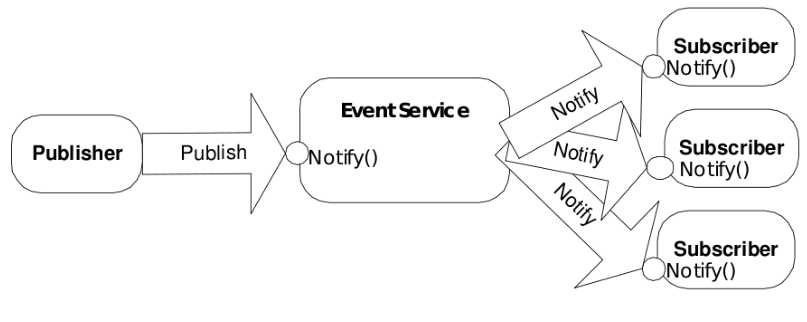
\includegraphics[width=\textwidth]{PublishSubscribe_Pattern.png}
%	\captionof{figure}{Sublish/Subscribe pattern}
%\end{center}


